\documentclass[titlepage]{article}
\usepackage[margin=3cm]{geometry}
\usepackage{datetime}
\usepackage{fontspec}
\usepackage{graphicx}
\usepackage{hyperref}
\usepackage{kotex}
\usepackage[lighttt]{lmodern}
\usepackage{listings}
\usepackage{tikz}
\usepackage{sectsty}
\usepackage[edges]{forest}
\usepackage{float}
\usepackage{flowchart}

\usepackage[headsepline]{scrlayer-scrpage}
\newcommand{\doctitle}{CSED101: Assignment 3}
\clearpairofpagestyles
\ohead{\thepage}
\ihead{\doctitle}

\usetikzlibrary{arrows}
\usetikzlibrary{fit}

\setmainhangulfont{Noto Serif CJK KR}[
  UprightFont=* Light, BoldFont=* Bold,
  Script=Hangul, Language=Korean, AutoFakeSlant,
]
\setsanshangulfont{Noto Sans CJK KR}[
  UprightFont=* DemiLight, BoldFont=* Medium,
  Script=Hangul, Language=Korean
]
\setmathhangulfont{Noto Sans CJK KR}[
  SizeFeatures={
    {Size=-6,  Font=* Medium},
    {Size=6-9, Font=*},
    {Size=9-,  Font=* DemiLight},
  },
  Script=Hangul, Language=Korean
]
\lstset{
  numbers=none, frame=single, showspaces=false,
  showstringspaces=false, showtabs=false, breaklines=true, showlines=true,
  breakatwhitespace=true, basicstyle=\ttfamily, keywordstyle=\bfseries, basewidth=0.5em
}
\allsectionsfont{\sffamily}

\title{\doctitle}
\author{무은재학부 손량 (20220323)}
\date{Last compiled on: \today, \currenttime}

\begin{document}

\makeatletter
\begin{titlepage}
  \begin{center}
    \vspace*{3cm}
    \Huge
    \textsf{\@title}

    \vspace{1.5cm}
    \LARGE
    \@author

    POVIS ID: \texttt{ryangsohn}

    \vspace{0.5cm}
    담당 교수: 윤은영 교수님

    \vfill
    \large
    \textit{``나는 이 프로그래밍 과제를 다른 사람의 부적절한 도움 없이 완수하였습니다.''}
  \end{center}
\end{titlepage}

\section{문제의 개요}

이 프로그램은 사다리 게임을 C언어로 구현한 것이다. 이 프로그램의 structure chart는 다음과 같다.\footnote{지면을 아끼기 위해 프로그램의 기능상 중요한 함수들 위주로 structure chart에 넣었다.}

\begin{figure}[H]
  \centering
  \begin{forest}
    for tree={
      draw,
      align=center,
      grow=east
    },
    forked edges,
    [ASSN3: 사다리 게임
      [\texttt{alloc\_2d}
      ]
      [\texttt{free\_ladder}
      ]
      [\texttt{generate\_ladder}
        [\texttt{draw\_vertical}
        ]
      ]
      [\texttt{save\_ladder}
      ]
      [\texttt{load\_ladder}
      ]
      [\texttt{print\_ladder}
        [\texttt{set\_output\_color}
        ]
        [\texttt{reset\_output\_color}
        ]
      ]
    ]
  \end{forest}
\end{figure}

\section{프로그램 구조 및 설명}

본 프로그램에서 사용한 알고리즘을 pseudocode로 나타내면 다음과 같다.

\begin{lstlisting}
set random seed to current time
infinite loop:
  print menu and get user input to menu_input
  if menu_input == 1:
    get number of participants, height, number of horizontal lines and filename
    allocate space for ladder info
    create ladder according to user input
    save the ladder to filename
    deallocate space for ladder info
  if menu_input == 2:
    get filename from user input
    load ladder from file
    if load failed:
      print error message
      continue
    allocate space for visited_map
    create variable y = -1, x = -1, print_full = false, current_source = 0
    infinite loop:
      if y != -1:
        print current coordinate
      print ladder with colors
      if y <= 0:
        if current_source != 0:
          if print_full:
            set print_full to false
            collect destinations for each alphabets
            print destinations
          else:
            print current destination
        mark all cells in visited_map as stale by setting the sign to minus
        get current_source from user input
        if current_source == 0:
          break
        if current_source == -1:
          re-allocate space for visited_map
          for every sources:
            simulate moving to the top
          set y = 0, x = 0, print_full = ture
          continue
      set y = height, x = (current_source - 1) * 2
      else:
        wait for user to press enter
      move one step
  if menu_input == 3:
    break
\end{lstlisting}

Flowchart로 나타내면 다음과 같다.

\begin{figure}[H]
  \centering
  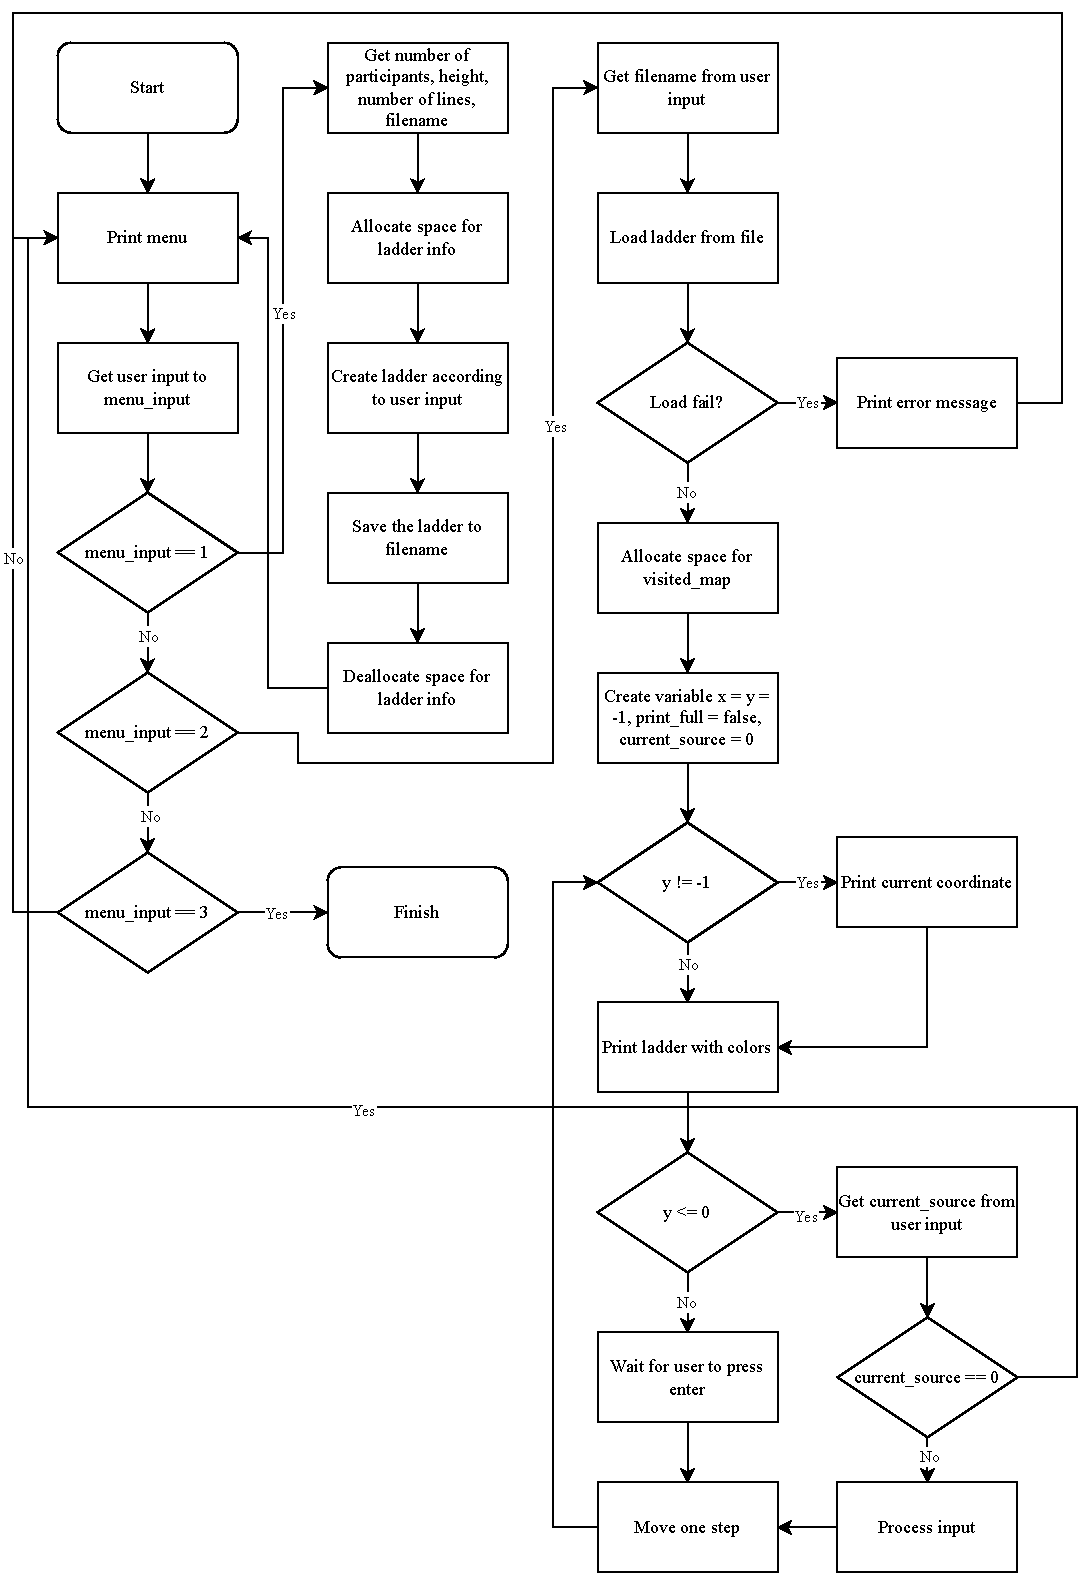
\includegraphics[width=0.9\linewidth]{flowchart.drawio.pdf}
\end{figure}

\section{프로그램 실행 방법과 예제}

첨부한 \texttt{assn3.c} 파일은 Linux, macOS 등의 UNIX 계열 OS에서 실행하는 것을 전제로 작성되었다.\footnote{Windows의 경우 WSL이나 Cygwin 등의 환경에서 실행할 수 있을 것이다.} \texttt{gcc} 컴파일러가 설치된 환경에서는 다음 명령어를 통해 코드를 컴파일할 수 있다.

\begin{lstlisting}
$ gcc -o assn3 assn3.c
\end{lstlisting}

\begin{figure}[H]
  \centering
  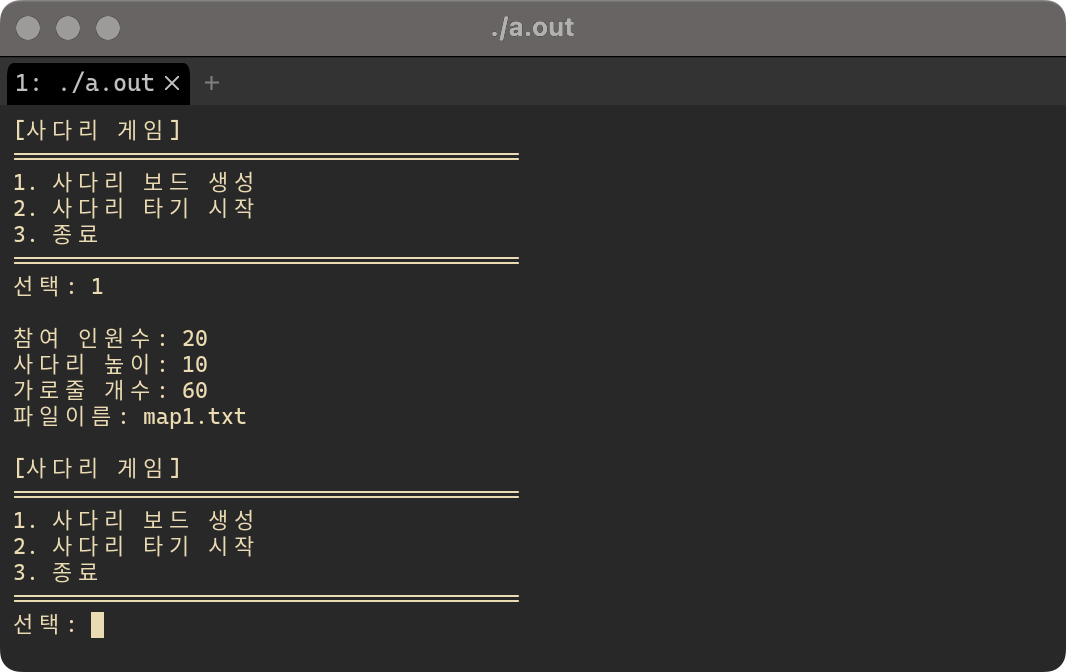
\includegraphics[width=0.7\linewidth]{generate.png}
  \caption{사다리 생성}
\end{figure}

\begin{figure}[H]
  \centering
  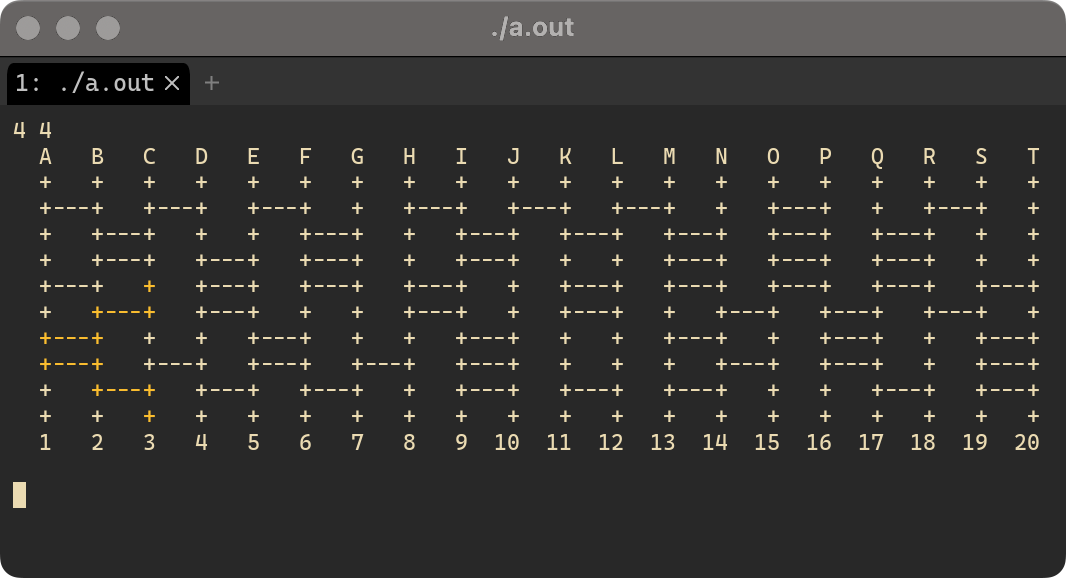
\includegraphics[width=0.7\linewidth]{play_progress.png}
  \caption{사다리 타기 게임 진행 중}
\end{figure}

\begin{figure}[H]
  \centering
  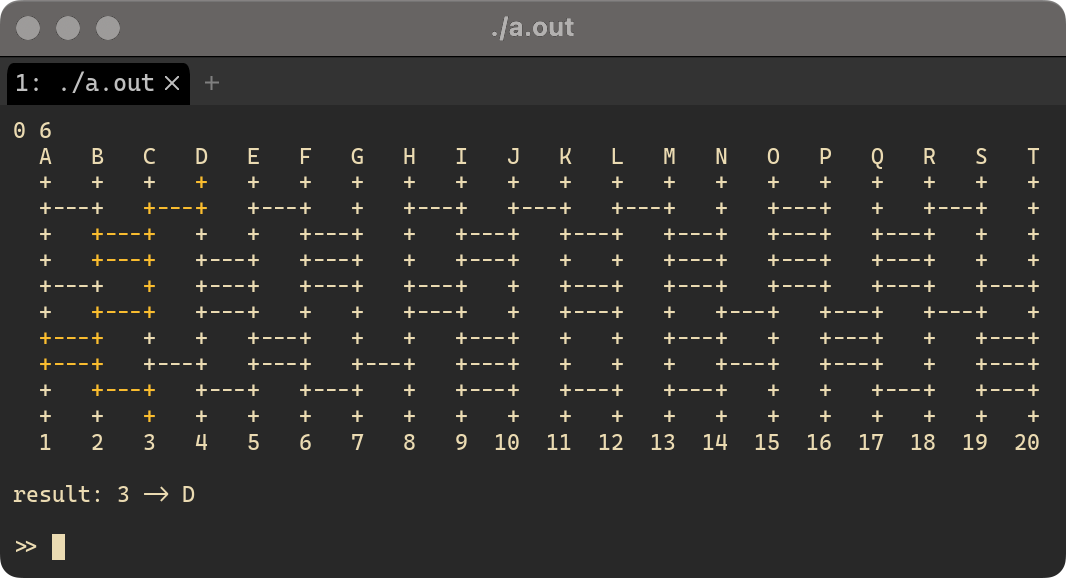
\includegraphics[width=0.7\linewidth]{play_finish_one.png}
  \caption{한 개의 출발지에서 도착한 경우}
\end{figure}

\begin{figure}[H]
  \centering
  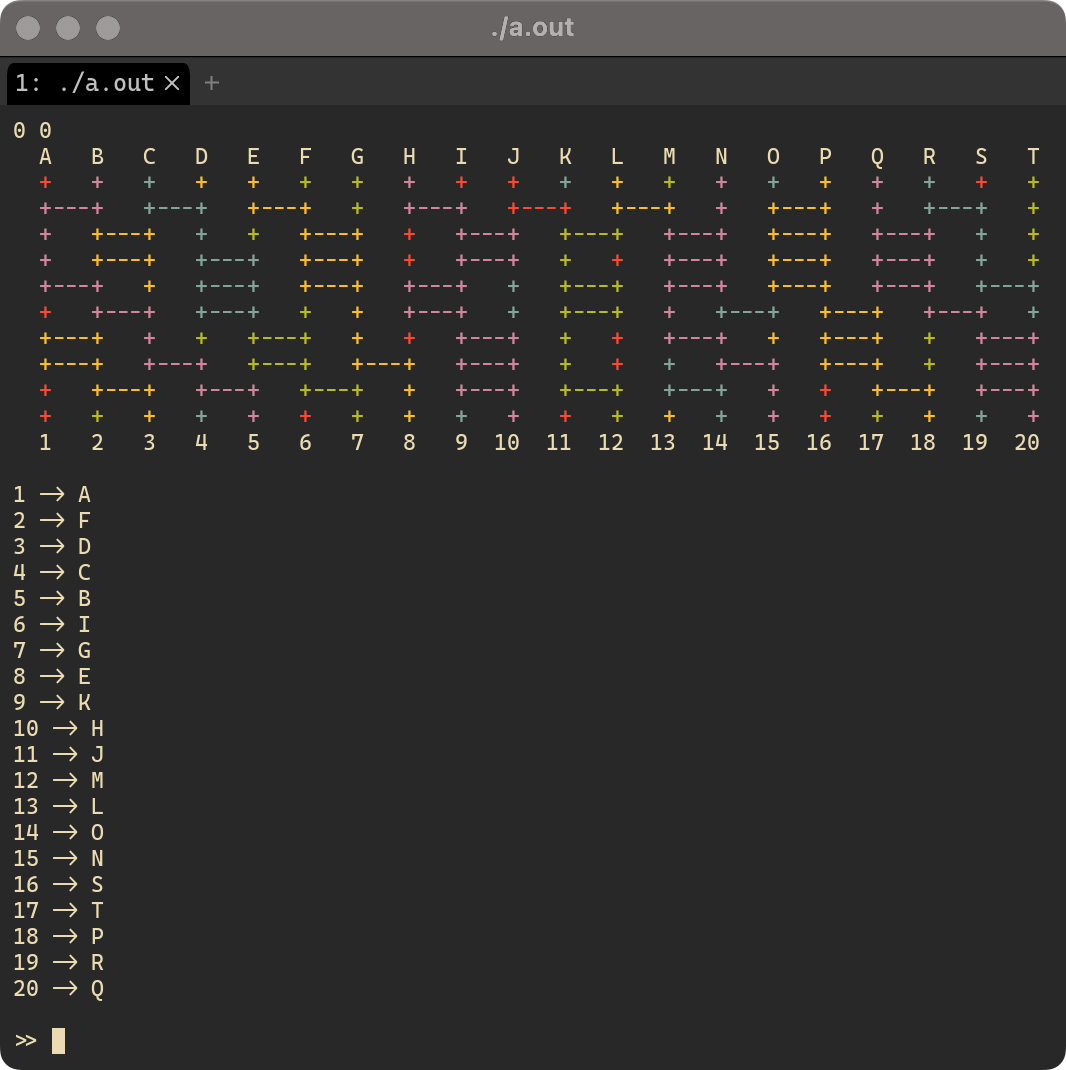
\includegraphics[width=0.7\linewidth]{play_finish_all.png}
  \caption{모든 출발지에서 사다리를 탄 결과}
\end{figure}

\section{토론}

\subsection{사다리의 무작위 생성}
사다리를 무작위로 생성하는 알고리즘은 가로줄의 좌표를 \texttt{rand} 함수를 사용하여 생성하고, 그 위치에 이미 가로줄이 있거나 옆에 가로줄이 있는 경우에는 다시 사다리의 위치를 뽑는 방식으로 구현하였다.

\subsection{사다리 타기 구현}
사다리 타기 과정에서는 현재 타고 있는 사다리에서의 위치 뿐만 아니라 지금까지 방문했던 위치들의 기록까지 저장해야 한다. 이를 구현하기 위해서 \texttt{visited\_map}이라는 배열을 생성하고 이를 관리하였다. \texttt{visited\_map} 배열은 사다리 정보를 저장하는 2차원 배열과 같은 크기를 가지고, 사다리 정보를 저장하는 배열의 각 원소에 대해서, 사다리의 그 부분을 방문했다면 마지막으로 방문했을 때의 시작점을 저장한다. 또한, 시작점을 저장하는 방식에는 두 가지 방법이 있는데, ``활성'' 상태와 ``비활성'' 상태이다. 사다리 타기 과정에서 1 이상의 입력을 받았을 때, 엔터를 누르면서 위로 올라가는 동안 방문했던 위치들에는 ``활성'' 상태로 저장된다. 이 위치들에는 \texttt{visited\_map}에서 시작점의 번호가 그대로 저장된다. 한편 ``비활성'' 상태로 저장된 위치들은 \texttt{visited\_map}에서 시작점의 번호가 음수 형태로 저장된다. 이는 이미 올라갔던 경로를 똑같은 시작점에서 지나갈 때 구분하기 위함이다. 사다리를 출력하는 \texttt{print\_ladder} 함수에서는 사다리 정보의 배열 뿐만 아니라 \texttt{visited\_map} 또한 받고, 이 배열에 저장된 시작점을 기반으로 색을 칠한다.

\section{결론과 개선 방향}

C언어를 활용하여 사다리 타기 프로그램을 작성하였다. 프로그램은 잘 동작하지만, 몇 가지 개선할 만한 점을 여기 적어 보았다.

\subsection{안전한 난수 생성}
어싸인 문서에서 보았듯 이번에 구현한 사다리 타기 프로그램은 간식 내기 등 사용자의 이득과 직접적으로 연관된 문제를 해결한다. 때문에 악의적인 사용자의 경우 이 프로그램을 이용하여 부당한 이득을 취하는 데 이용할 가능성이 있다. 가장 우려할 만한 문제는 이 프로그램에서 사용하는 \texttt{rand} 함수이다. C언어의 \texttt{rand} 함수는 대부분의 플랫폼에서 그 자체로 취약할 뿐만 아니라, 이 프로그램이 시작할 때 시드를 현재 시간을 기준으로 설정한다. 악의적인 사용자의 경우 timing attack을 수행하여 자신이 원하는 사다리 배치가 \texttt{generate\_ladder}에서 생성되도록 할 수 있다. 이러한 문제를 해결하기 위해 \texttt{/dev/urandom}과 같은 암호학적으로 안전한 난수 생성기를 사용하여 사다리를 생성하도록 보완할 필요가 있을 것이다.

\subsection{메모리 최적화}
이 프로그램에서 사다리 정보를 저장하는 데에는 게임의 참여하는 사람 수와 사다리의 높이의 곱에 비례하는 크기의 메모리를 사용한다. 하지만 이렇게 저장된 사다리 정보에서 중요한 것은 가로줄의 위치들이고, 세로줄의 위치와 같은 정보는 굳이 저장할 필요가 없다. 2차원 배열 대신 적당한 자료구조에 가로줄의 위치만 저장한다면 메모리 사용량을 줄일 수 있을 것이다.

\end{document}
